%20 min preso!
\documentclass[xcolor=table]{beamer}
\usepackage{beamerthemesplit}
\usepackage{wrapfig}
\usetheme{SPbGU}
\usepackage{pdfpages}
\usepackage{amsmath}
\usepackage{cmap}
\usepackage[T2A]{fontenc}
\usepackage[utf8]{inputenc}
\usepackage[english]{babel}
\usepackage{indentfirst}
\usepackage{amsmath}
\usepackage{tikz}
\usepackage{multirow}
\usepackage[noend]{algpseudocode}
\usepackage{algorithm}
\usepackage{algorithmicx}
\usepackage{fancyvrb}
\usetikzlibrary{calc}
\usetikzlibrary{shapes,arrows}
\usetikzlibrary{arrows,automata}
\usetikzlibrary{positioning}

\usepackage{tabularx}
\newcolumntype{Y}{>{\raggedleft\arraybackslash}X}


\newtheorem{mytheorem}{Theorem}
\renewcommand{\thealgorithm}{}

\newcommand{\tikzmark}[1]{\tikz[overlay,remember picture] \node (#1) {};}
\def\Put(#1,#2)#3{\leavevmode\makebox(0,0){\put(#1,#2){#3}}}

\tikzset{
    state/.style={
           rectangle,
           rounded corners,
           draw=black, very thick,
           minimum height=2em,
           inner sep=2pt,
           text centered,
           },
}

\beamertemplatenavigationsymbolsempty

\title[ТФЯ на практике]{Теория формальных языков на практике}
\subtitle[]{Открытая лекция Computer Science Center}
% То, что в квадратных скобках, отображается в левом нижнем углу.
\institute[JB Research, СПбГУ]{
Лаборатория языковых инструментов JetBrains \\
Санкт-Петербургский государственный университет \\
Математико-механический факультет }

% То, что в квадратных скобках, отображается в левом нижнем углу.
\author[Семён Григорьев]{Семён Григорьев}

\date{18 октября 2019г.}

\definecolor{orange}{RGB}{179,36,31}

\begin{document}
{
\begin{frame}[fragile]
  \begin{tabular}{p{2.5cm} p{5.5cm} p{2cm}}
   \begin{center}
      
\includegraphics[height=1.5cm]{pictures/jetbrainsResearch.pdf}
    \end{center}
    &
    \begin{center}
      
\includegraphics[height=1.5cm]{pictures/csc.jpg}
    \end{center}
    &
    \begin{center}
      
\includegraphics[height=1.5cm]{pictures/SPbGU_Logo.png}
    \end{center}
  \end{tabular}
  \titlepage
\end{frame}
}

\begin{frame} \frametitle{Кто я}
   \begin{itemize}
     \item Семён Григорьев
     \begin{itemize}
       \item rsdpisuy@gmail.com
       \item semyon.grigorev@jetbrains.com
       \item \url{https://research.jetbrains.org/researchers/gsv}
     \end{itemize}
     \item Исследовательская группа на Математико-Механическом факультете СПбГУ
     \item Исследовательская группа в лаборатории языковых инструментов JetBrains Research: : \textbf{\url{https://research.jetbrains.org/groups/plt_lab}}
     \item Сферы интереснов
      \begin{itemize}
        \item Теория формальных языков
        \item \textbf{Применение теории формальных языков для решения прикладных задач}
      \end{itemize}
    \end{itemize}

\end{frame}

\begin{frame} \frametitle{Поиск путей с ограничениями в терминах формальных языков}
\begin{itemize}
\item Конечный ориентированный граф с метками на рёбрах $\mathcal{G} = (V,E,L)$
\item Путь --- это слово в алфавите $L$ $\omega(p) = \omega(v_0 \xrightarrow{l_0} v_1 \xrightarrow{l_1} \dots \xrightarrow{l_{n-1}} v_n ) = l_0 \cdot l_1 \cdot \ldots \cdot l_{n-1}$
\item Язык $\mathcal{L}$ (над алфавитом $L$)
\end{itemize}
\pause
\begin{itemize}
  \item Задача достижимости: $Q=\{(v_i,v_j) \ | \ \exists p = v_i \dots v_j, \omega(p) \in \mathcal{L}\}$
  \item Задача поиска путей: $Q=\{p \ | \ \omega(p) \in \mathcal{L}\}$
  \begin{itemize}
    \item Один путь, все пути, кратчайший путь\dots
  \end{itemize}
\end{itemize}

\end{frame}

\begin{frame} \frametitle{Поиск путей с контекстно-свободными ограничениями}
\begin{itemize}
\item $\mathcal{L}$ --- контекстно-свободный язык (КС язык)
\item $G_{\mathcal{L}} = (N,\Sigma,R,S)$
\item Задача достижимости: $Q=\{(v_i,v_j) \ | \ \exists p = v_i \dots v_j, S \xrightarrow[G_{\mathcal{L}}]{*} \omega(p) \}$
\item Задача поиска путей: $Q=\{p \ | \ S \xrightarrow[G_{\mathcal{L}}]{*} \omega(p)\}$
\end{itemize}

\end{frame}

\begin{frame} \frametitle{Пример КС запроса}
\begin{center}
  \begin{tabular}{  c  c  }
      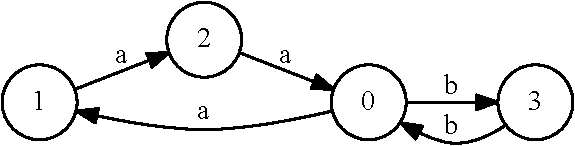
\includegraphics[width=0.45\textwidth]{pictures/input.pdf}
      &
  $

  \begin{array}{rl}
     & S \rightarrow a \ S \ b \\
     & S \rightarrow Middle \\
     & Middle \rightarrow a \ b
  \end{array}

  $
  \\
  Входной граф
  &
  Запрос: язык $\{a^nb^n \ | \ n > 0 \}$

  \end{tabular}

\end{center}

\pause

\vspace{0.5cm}
Пример путей: \\
$2 \xrightarrow{a} 0 \xrightarrow{b} 3$ \\
$1 \xrightarrow{a} 2 \xrightarrow{a} 0 \xrightarrow{b} 3 \xrightarrow{b} 0$ \\
$p_1 = 0 \xrightarrow{a} 1 \xrightarrow{a} 2 \xrightarrow{a} 0 \xrightarrow{b} 3 \xrightarrow{b} 0 \xrightarrow{b} 3$ \\
$p_2 = 0 \xrightarrow{a} 1 \xrightarrow{a} 2 \xrightarrow{a} 0 \xrightarrow{a} 1 \xrightarrow{a} 2 \xrightarrow{a} 0 \xrightarrow{b} 3 \xrightarrow{b} 0 \xrightarrow{b} 3 \xrightarrow{b} 0 \xrightarrow{b} 3 \xrightarrow{b} 0$ \\
$\dots$

\end{frame}


\begin{frame} \frametitle{Контекстно-свободная достижимость для статического анализа кода}

  \begin{itemize}
      \item \emph{Thomas Reps et al.} ``Precise interprocedural dataflow analysis via graph reachability.'' 1995
      \item \emph{Jakob Rehof and Manuel Fahndrich.} ``Type-base flow analysis: from polymorphic subtyping to CFL-reachability.'' 2001
      \item \emph{Dacong Yan et al.} ``Demand-driven context-sensitive alias analysis for Java.'' 2011
      \item \emph{Qirun Zhang et al.}  ``Efficient subcubic alias analysis for C.'' 2014
      \item \emph{Kai Wang et. al.} ``Graspan: a single-machine disk-based graph system for interprocedural static analyses of large-scale systems code.'' 2017
      \item \emph{Qirun Zhang and Zhendong Su.} ``Context-sensitive data-dependence analysis via linear conjunctive language reachability.'' 2017
  \end{itemize}

\end{frame}


\begin{frame}[fragile] \frametitle{Контекстно-свободная достижимость для графовых баз данных}

  \begin{itemize}
      \item \emph{M. Yannakakis} ``Graph-theoretic methods in database theory.'' 1990
      \item \emph{C. Barrett, R. Jacob, and M. Marathe} ``Formal-language-constrained path problems.'' 2000
      \item \emph{Sevon P., Eronen L.} ``Subgraph queries by context-free grammars.'' 2008
      \item \emph{Hellings J.} ``Conjunctive context-free path queries.'' 2014
      \item \emph{Zhang X. et al.} ``Context-free path queries on RDF graphs.'' 2016
      \item \emph{Jochem Kuijpers, George Fletcher, Nikolay Yakovets, and Tobias Lindaaker} ``An Experimental Study of Context-Free Path Query Evaluation Methods.'' 2019
  \end{itemize}

\end{frame}



\begin{frame}[fragile] \frametitle{Субкубический алгоритм для решения задачи КС-достижимости}

  \begin{itemize}
      \item \emph{L. G. Valiant} ``General context-free recognition in less than cubic time.'' 1975
      \item \emph{Ph. G. Bradford} ``Efficient exact paths for dyck and semi-dyck labeled path reachability.'' 2017
      \item \emph{Krishnendu Chatterjee} ``Optimal Dyck reachability for data-dependence and alias analysis.'' 2017
  \end{itemize}

\end{frame}



\end{document}
